\section{\textsf{Simulation}}
    The simulation has be created using the CST software in order to implement a configuration such as shown in \cite{zhang_design_2023}.

    \subsection{\textsf{CST Implementation}}
        The vertical layout implemented in CST consists of a three layer structure:
        \begin{itemize}
            \item Dielectric substrate
            \item Air
            \item Metal Backplate
        \end{itemize}

        The dielectric substrate will also embody a metallic component made of the same material as the metal backplate; copper
        (5.96 \mu $10^7$ S/m).

        At first the FR-4 substrate is placed without the metal resonance layer and then the two other layers - all below Z=0,
        turning on the orthographic side view the layout is as (\ref{img:layout}).
        \begin{figure}[h]
            \centering
            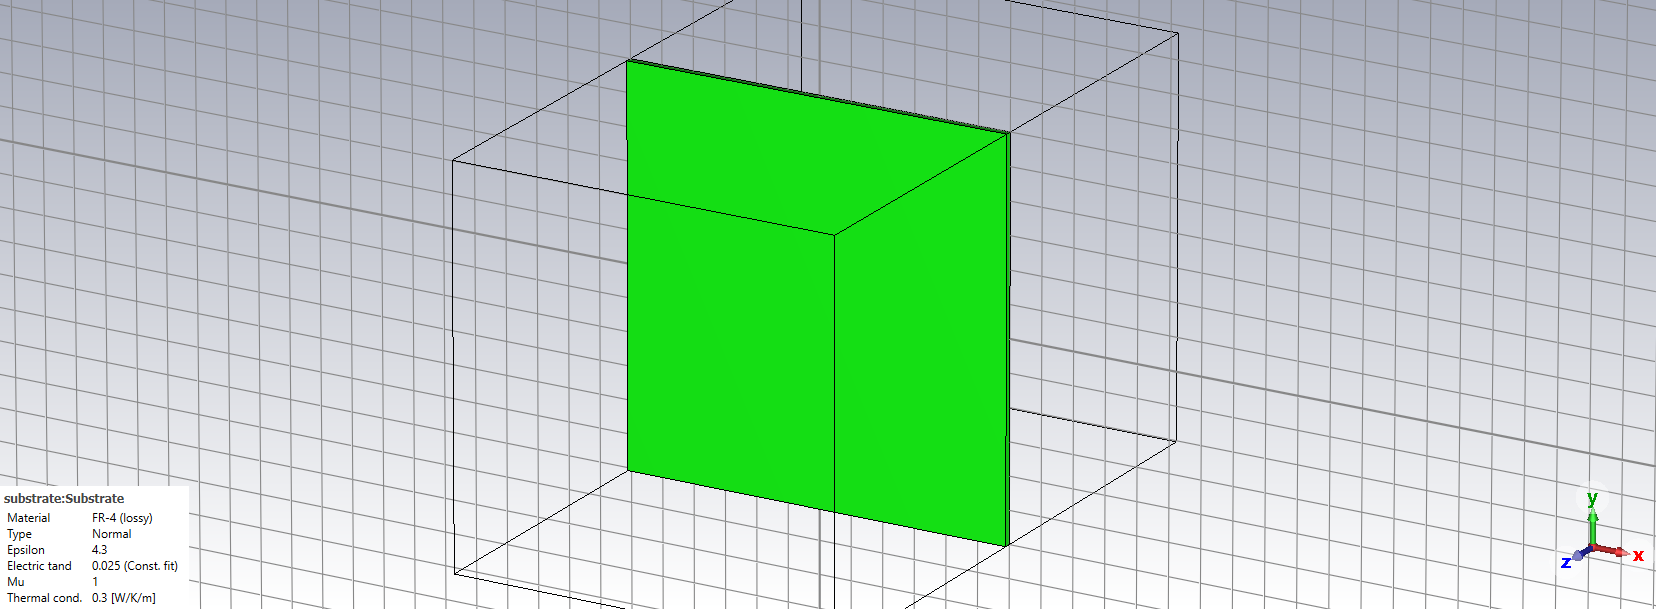
\includegraphics[width=0.4\textwidth]{substrate.png}\hfil
            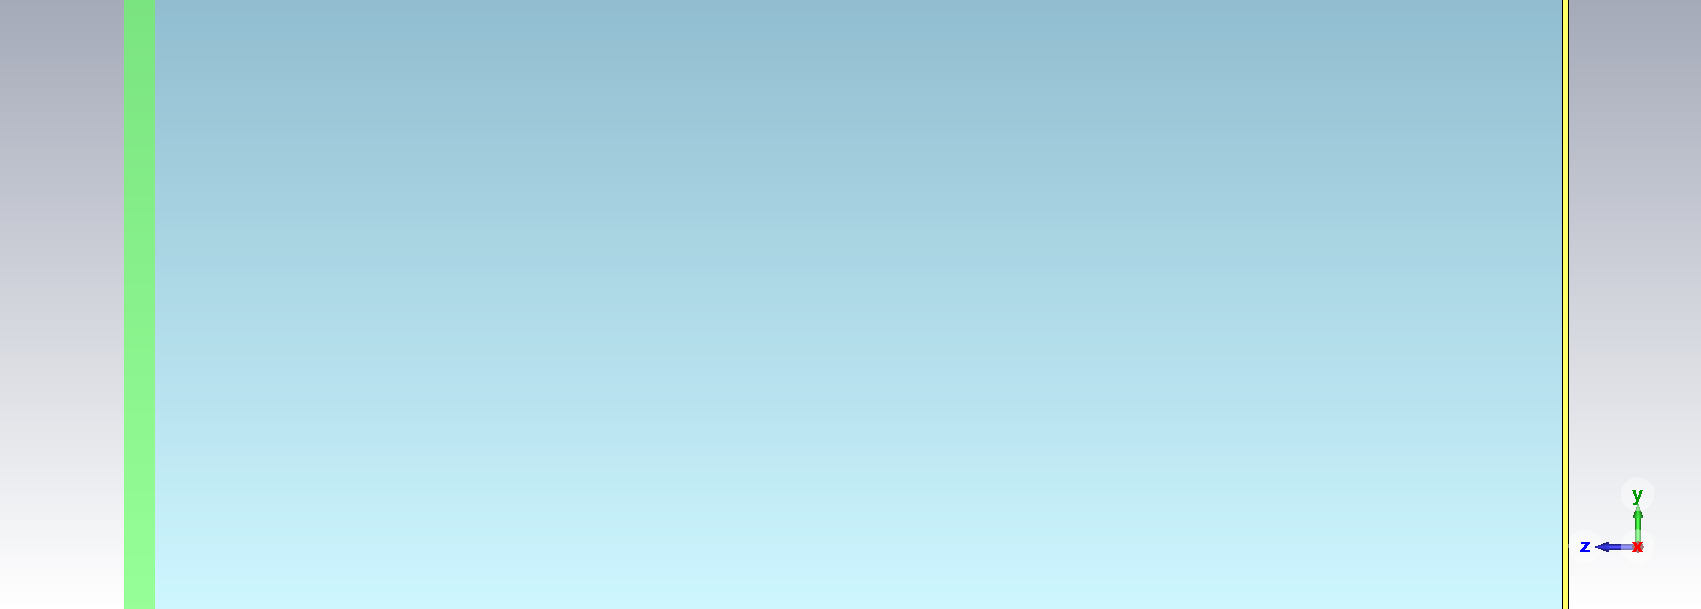
\includegraphics[width=0.4\textwidth]{verticaLayout.png}
            \caption{Basic Vertical Layout}
            \label{img:layout}
        \end{figure}

        Then the ring is added so that is of the same material and thickness as the backplate and lays
        on top of the dielectric substrate as shown in (\ref{img:ring}) 
        \begin{figure}[h]
            \centering
            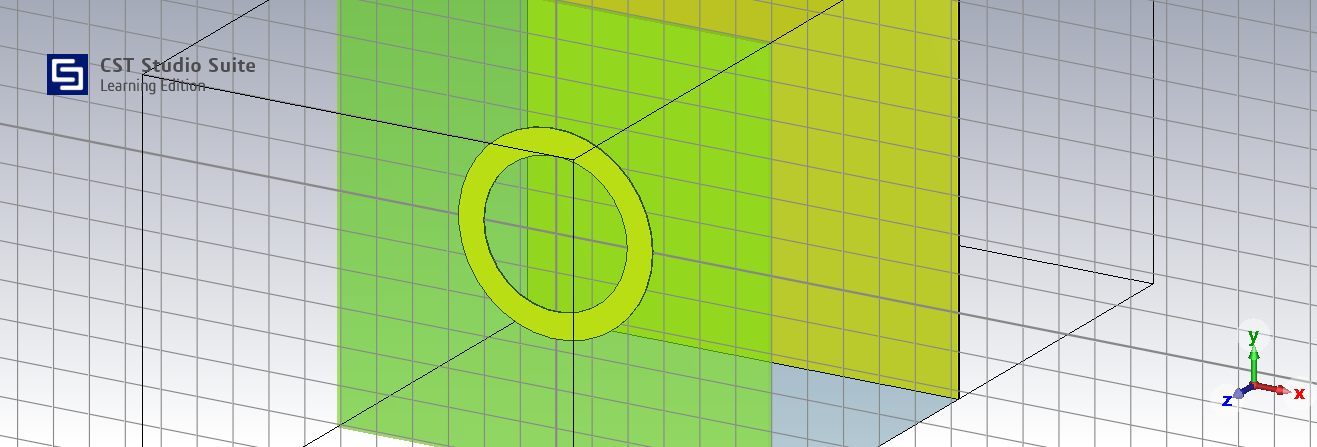
\includegraphics[width=0.6\textwidth]{ring.png}
            \caption{Ring Resonator}
            \label{img:ring}
        \end{figure}

        The assumption made is that both the arrow body and point are $\alpha=0.5mm$ of width.
        In order to accurately place all the curve points that define the arrow some basic calculations
        shall be made. The two points of the arrow base lie exactly on the arc of the ring and are 
        equidistant from curve y=x so the in order to find their cartesian coordinates the following
        system shall be solved. 

        \begin{lstlisting}[frame=single, numbers=left, style=Matlab-Pyglike]
            syms x1 x2

            eq1 = 2*(x1 - x2)^2 == .5^2;
            eq2 = sqrt(x2^2 + x1^2) == 2.7;

            sol = solve([eq1, eq2], [x1 x2]);
            disp([sol.x1 sol.x2]);  
        \end{lstlisting}
        
        \begin{equation}
            \label{eq:xysys}
            \displaystyle \begin{array}{l} 
                \left(\begin{array}{cc} 
                    \sigma_3 -\frac{2916\,\sigma_1 }{1433} & -\sigma_1 \\
                    \sigma_4 -\frac{2916\,\sigma_2 }{1433} & -\sigma_2 \\
                    \frac{2916\,\sigma_1 }{1433}-\sigma_3  & \sigma_1 \\
                    \frac{2916\,\sigma_2 }{1433}-\sigma_4  & \sigma_2  
                \end{array}\right)\\
                \mathrm{}\\
                \textrm{where}\\
                \mathrm{}\\
                \;\;\sigma_1 =\sqrt{\frac{729}{200}-\frac{7\,\sqrt{59}}{80}}\\
                \mathrm{}\\
                \;\;\sigma_2 =\sqrt{\frac{7\,\sqrt{59}}{80}+\frac{729}{200}}\\
                \mathrm{}\\
                \;\;\sigma_3 =\frac{400\,{{\left(\frac{729}{200}-\frac{7\,\sqrt{59}}{80}\right)}}^{3/2} }{1433}\\
                \mathrm{}\\
                \;\;\sigma_4 =\frac{400\,{{\left(\frac{7\,\sqrt{59}}{80}+\frac{729}{200}\right)}}^{3/2} }{1433}
            \end{array}
        \end{equation}

        Then the arrow is mirrored against the X, the Y and the XY planes in order to reach all four 
        sides of the cell, then the face is covered with copper and a height of d=0.035mm is also 
        attributed, which is why it was important to move all other layers below Z=0. 
        \begin{figure}[h]
            \centering
            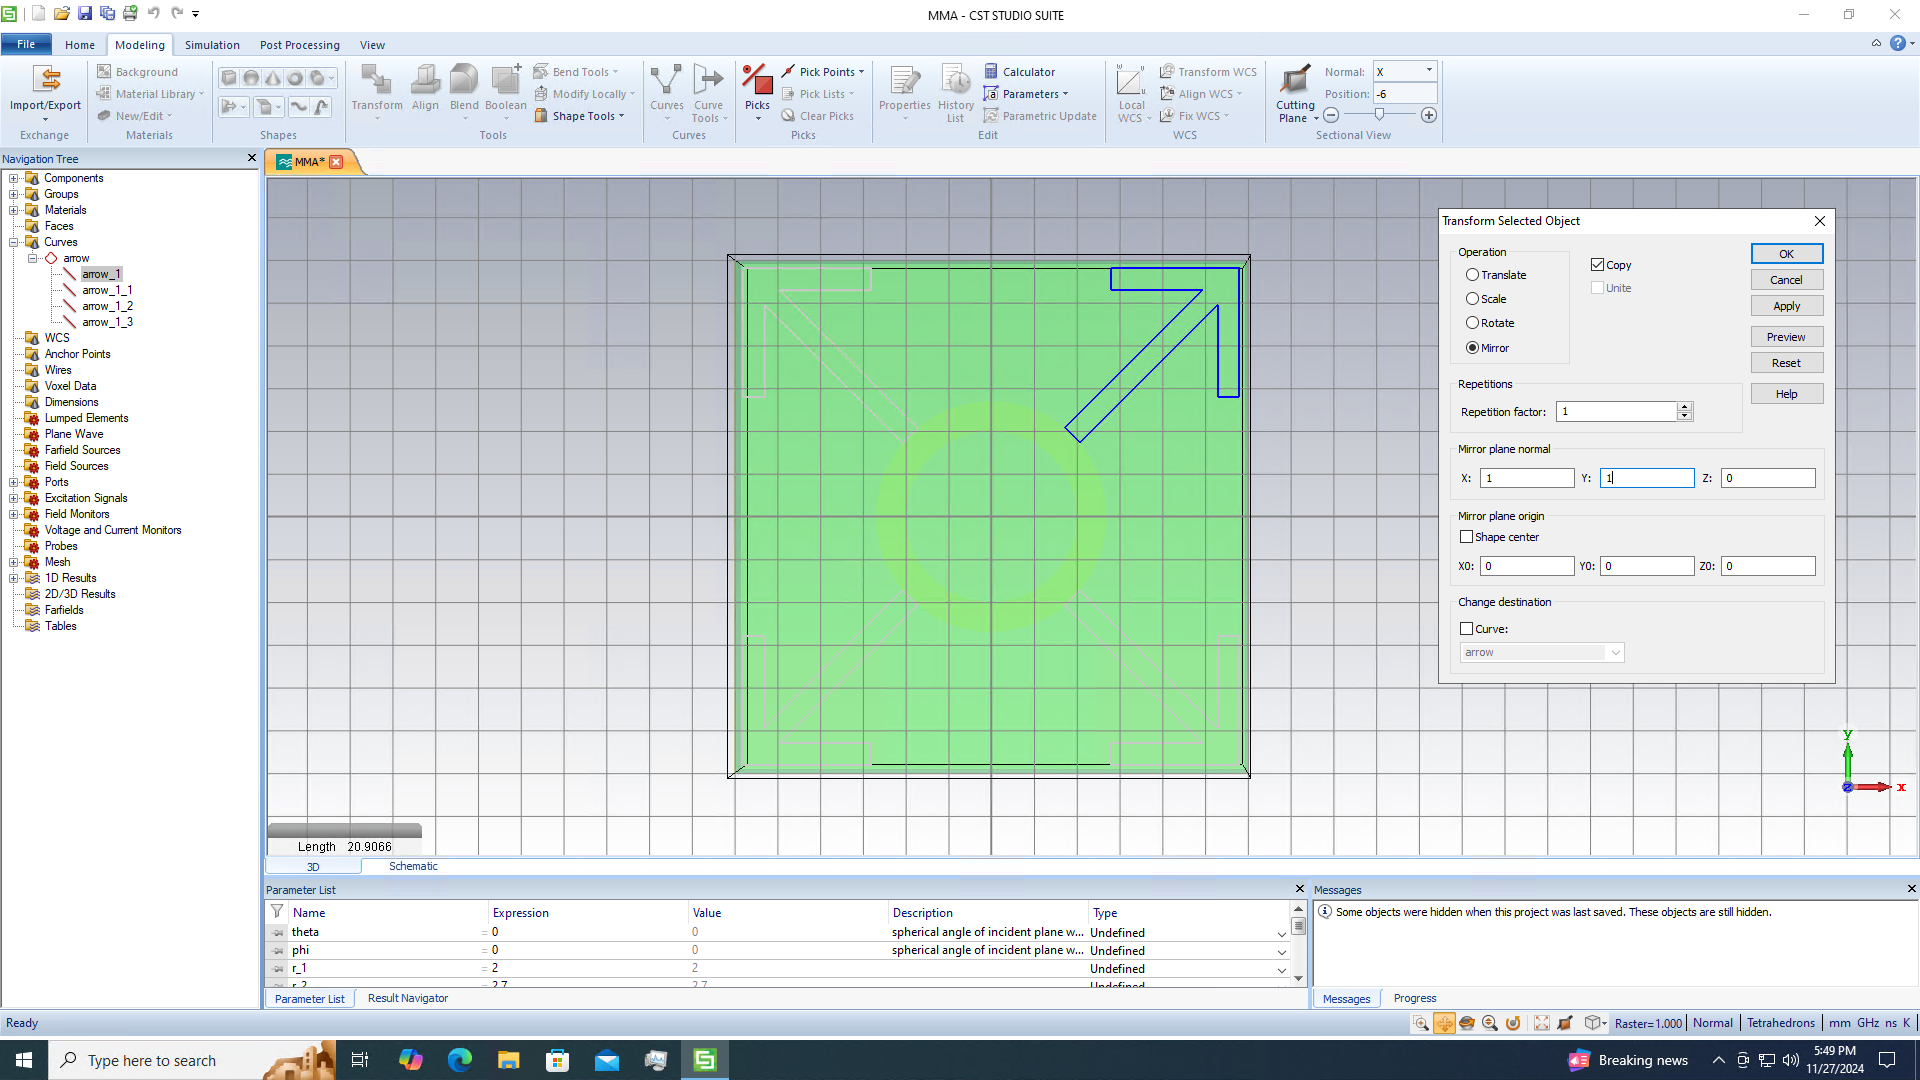
\includegraphics[width=.4\textwidth]{mirroredArrows.png}\hfil
            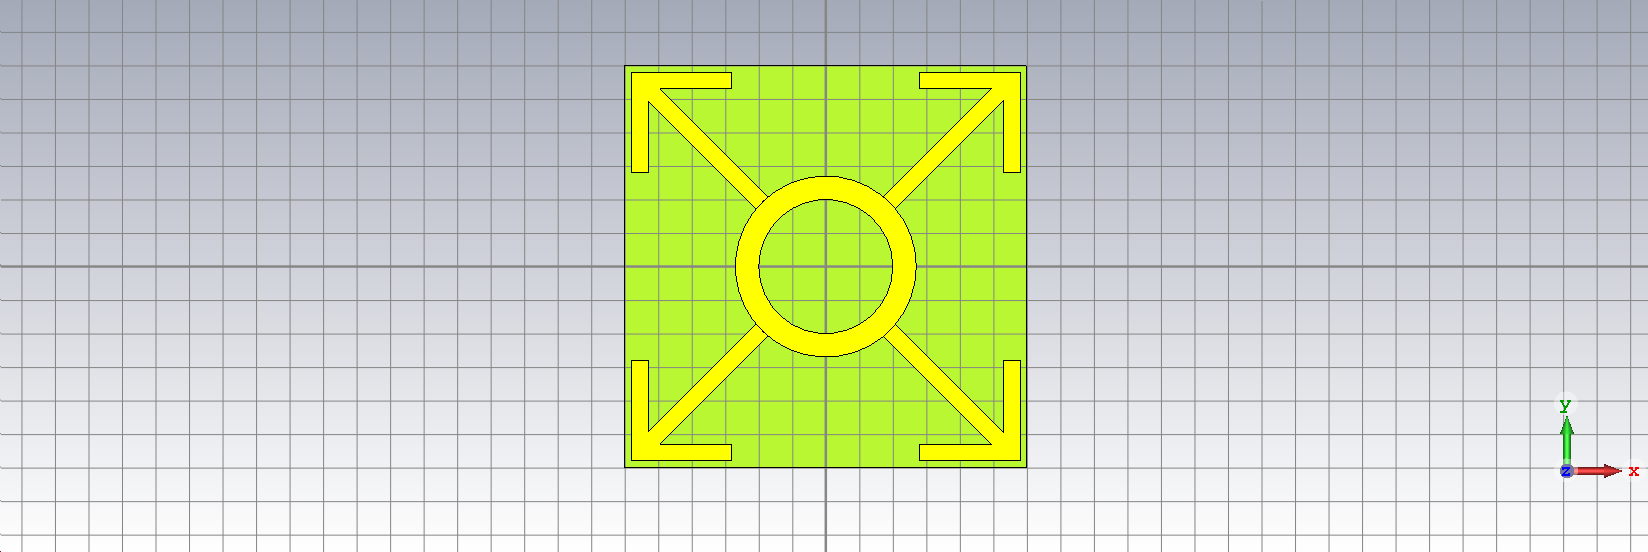
\includegraphics[width=.4\textwidth]{RingAndArrows.png}
            \caption{Mirroring Arrow and Cover}
            \label{img:mirrorAndCover}
        \end{figure}

        The following is a series of cuts in the resonance layer (boolean subtractions)
        in order to add the resistors between the copper faces.
        \begin{figure}[h]
            \centering
            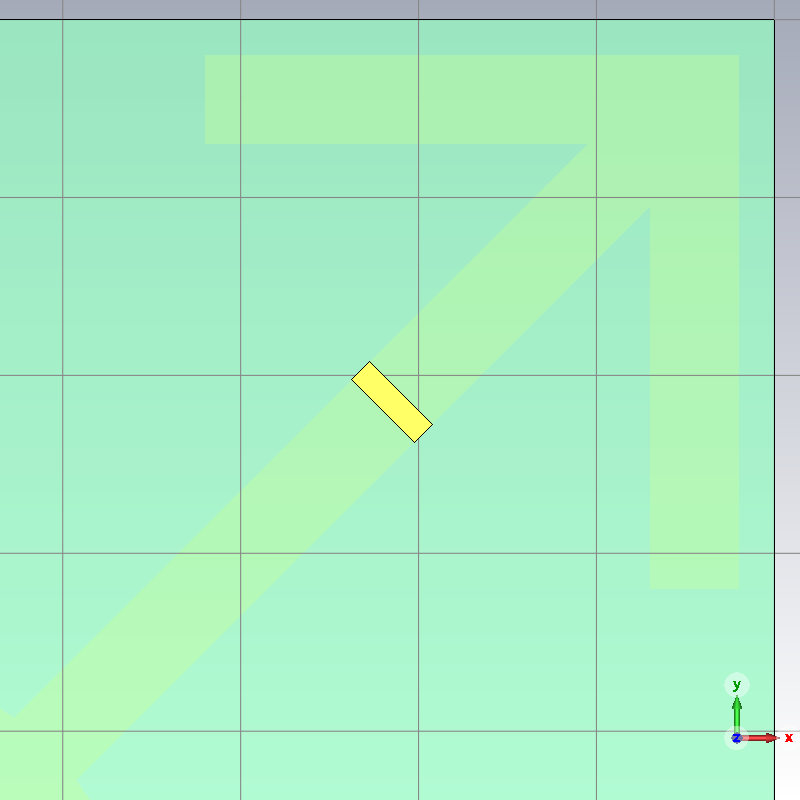
\includegraphics[width=.4\textwidth]{subtract.png}\hfil
            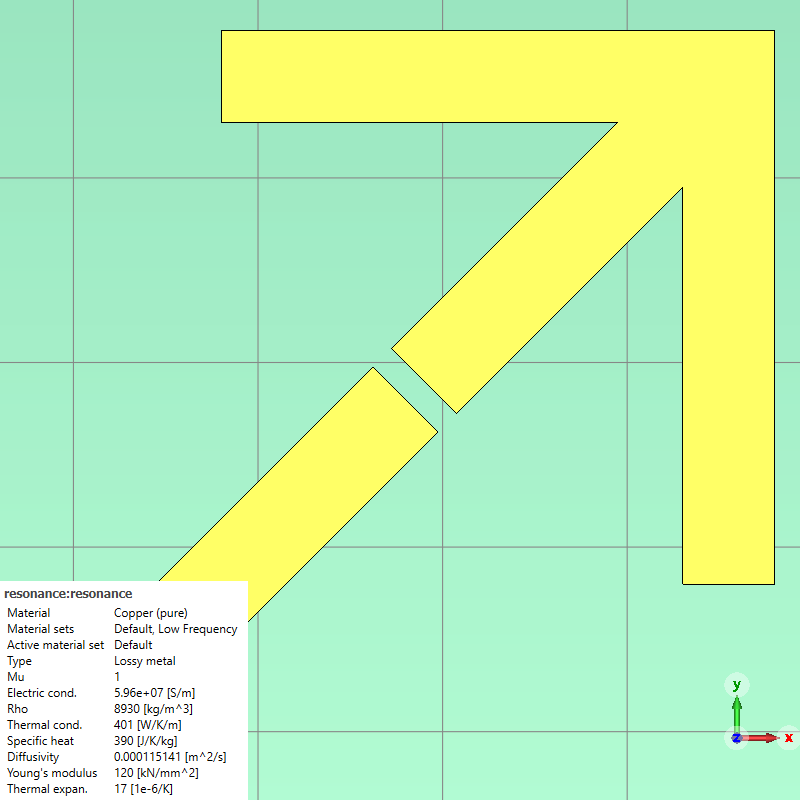
\includegraphics[width=.4\textwidth]{subtracted.png}
            \caption{Cuts Near the Arrows}
            \label{img:arrowCuts}
        \end{figure}

        \begin{figure}[h]
            \centering
            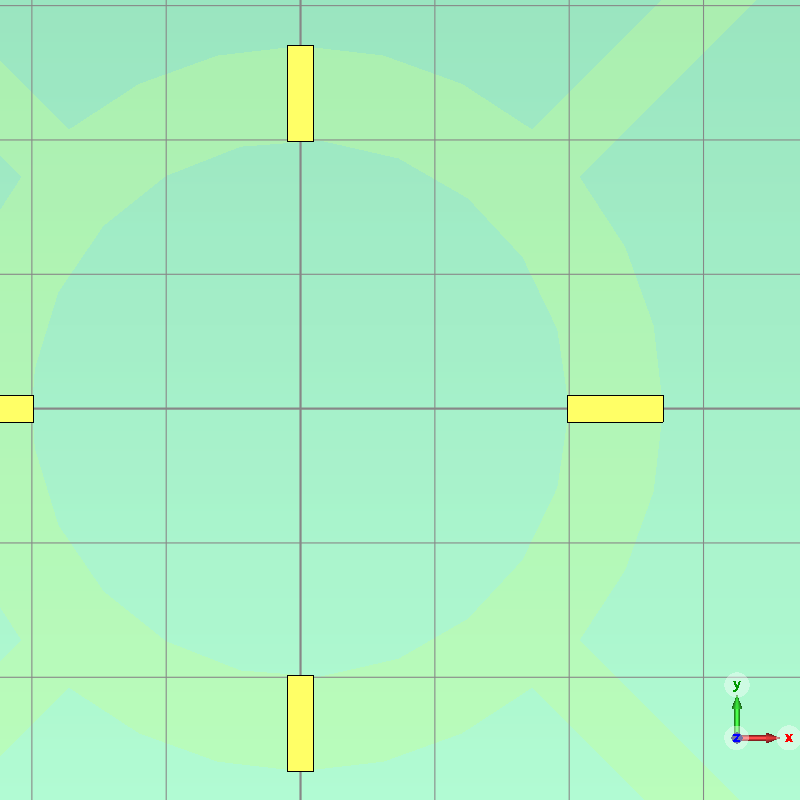
\includegraphics[width=.4\textwidth]{subtractRing.png}\hfil
            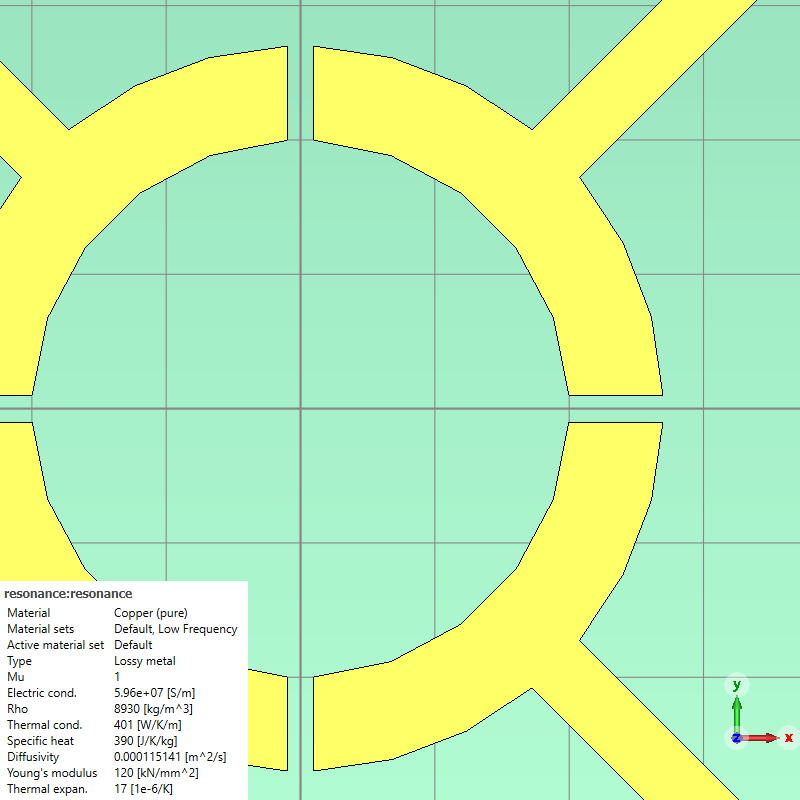
\includegraphics[width=.4\textwidth]{subtractedRing.png}
            \caption{Cuts Near the Ring}
            \label{img:ringCuts}
        \end{figure}

        Then the resistors are added connecting to the center points of the faces
        created by the previous subtractions \ref{img:resistors} (it is important to state that performance
        may be reduced in this implementation as better absorbance may be observed
        if the connection height is: $d=0.035mm$).
        \begin{figure}[h]
            \centering
            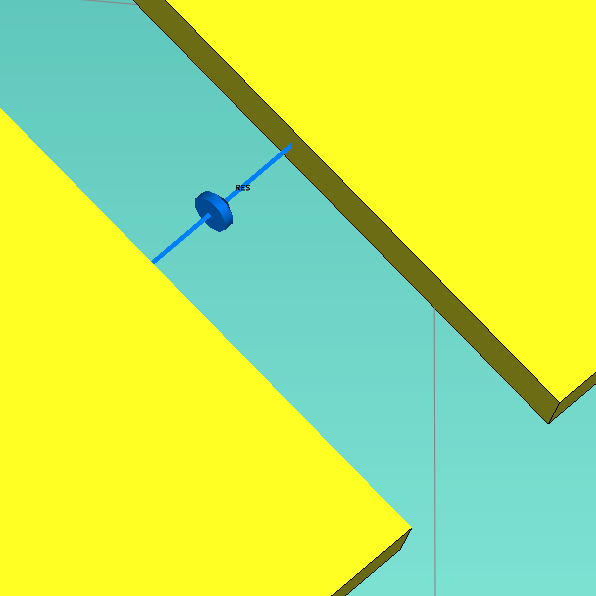
\includegraphics[width=0.5\textwidth]{faceCenterPoint.png}
            \caption{Resistor Placement}
            \label{img:resistors}
        \end{figure}

        Now to perform a simulation using the frequency solver in CST, the boundaries will be periodic
        along the XY plate free space conditions will be added along the Z axis.
        The Mesh that ends up being calculated is as \ref{img:RingAndArrowMesh}
        \begin{figure}[h]
            \centering
            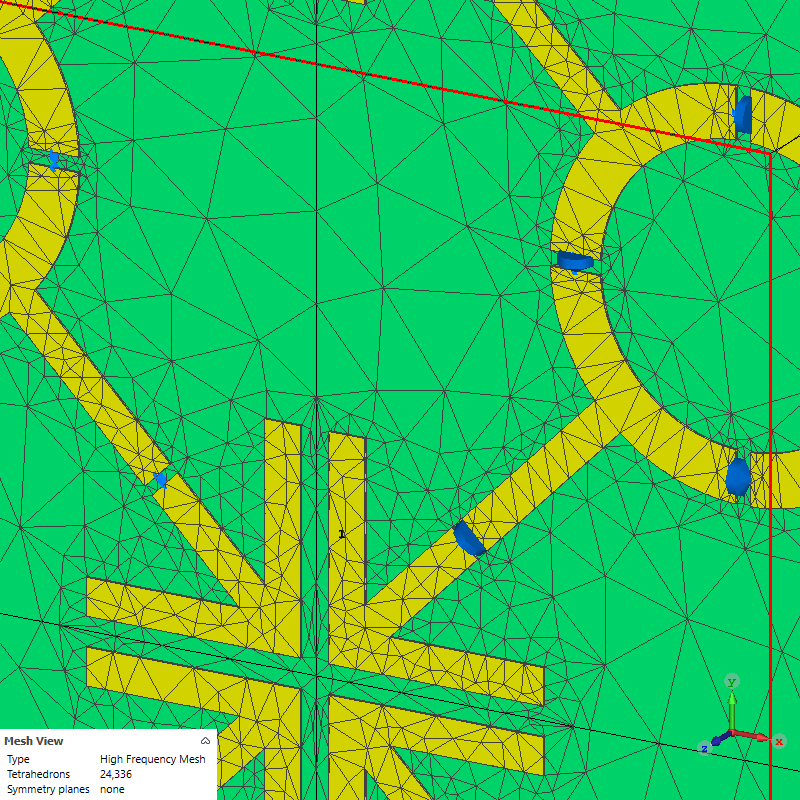
\includegraphics[width=0.5\textwidth]{mesh.png}
            \caption{Ring Mesh for reference}
            \label{img:RingAndArrowMesh}
        \end{figure}

        In the figure for the Electrical field absorbance the surfaces can be observed for $Z_{max}1$
        as in (\ref{img:E_Zmax1}).
        \begin{figure}[h]
            \centering
            \embedvideo{
                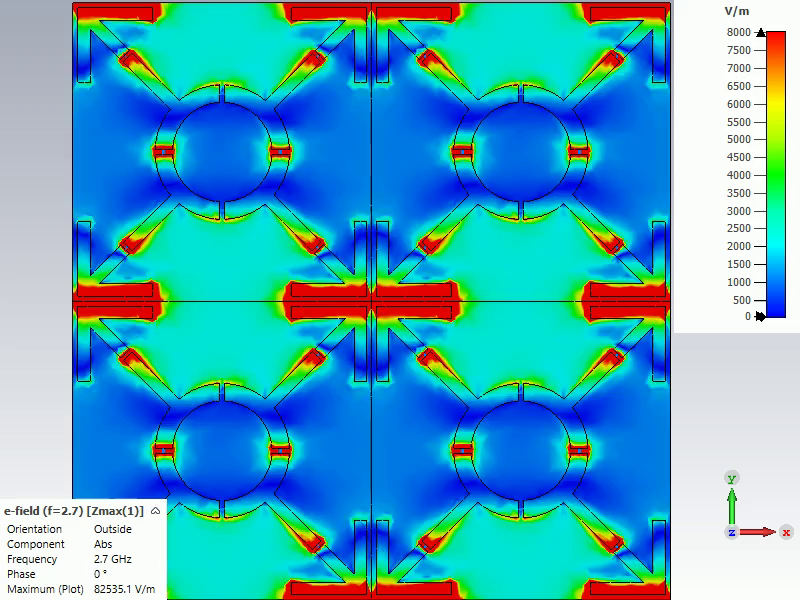
\includegraphics[page=1, width=0.22\textwidth]{E_Zmax1_027e2MHz.png}
            }{video/E_Zmax1_027e2MHz.mkv} \hfil
            \embedvideo{
                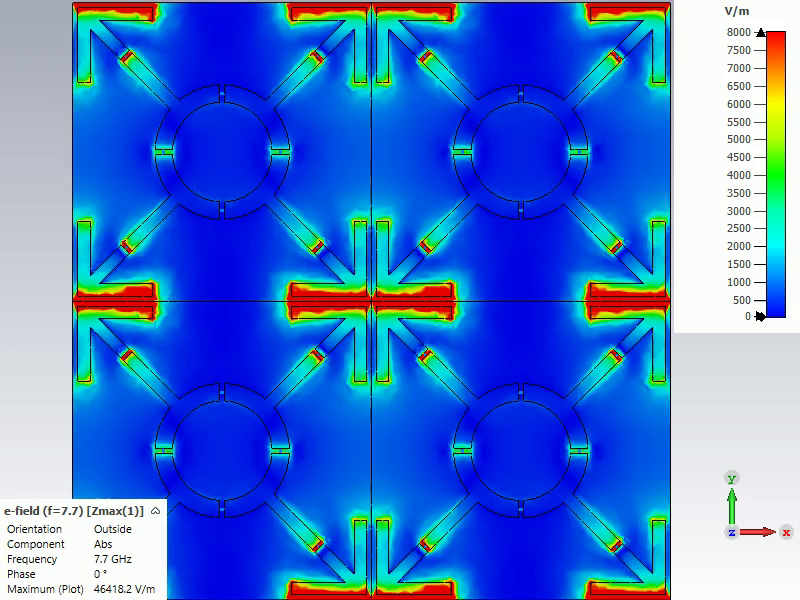
\includegraphics[page=1, width=0.22\textwidth]{E_Zmax1_077e2MHz.png}
            }{video/E_Zmax1_077e2MHz.mkv} \hfil
            \embedvideo{
                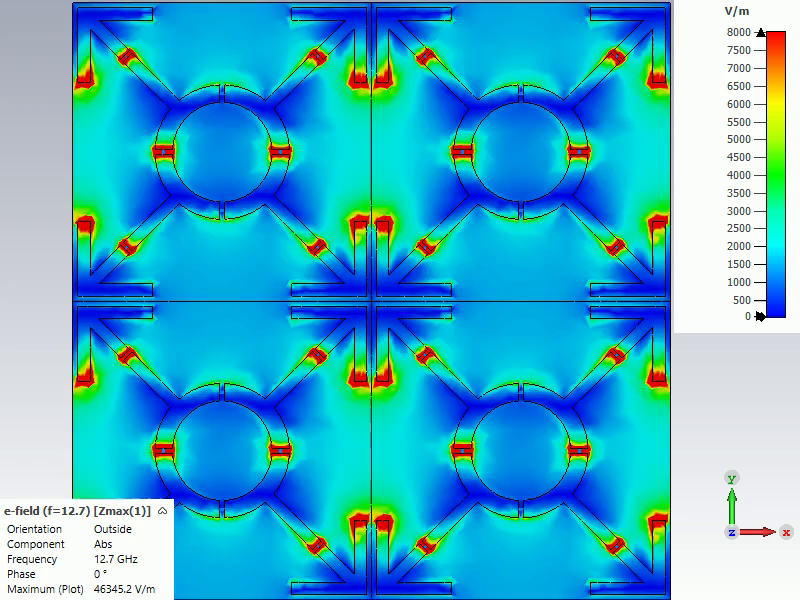
\includegraphics[page=1, width=0.22\textwidth]{E_Zmax1_127e2MHz.png}
            }{video/E_Zmax1_127e2MHz.mkv}

            \caption{Electrical Field for [2.7, 7.7, 12.7] GHz $Z_{max}(1)$}
            \label{img:E_Zmax1}
        \end{figure}

        As well as for the $Z_{max}2$ the Electrical field can be observed as in (\ref{img:E_Zmax2}).
        \begin{figure}[h]
            \centering
            \embedvideo{
                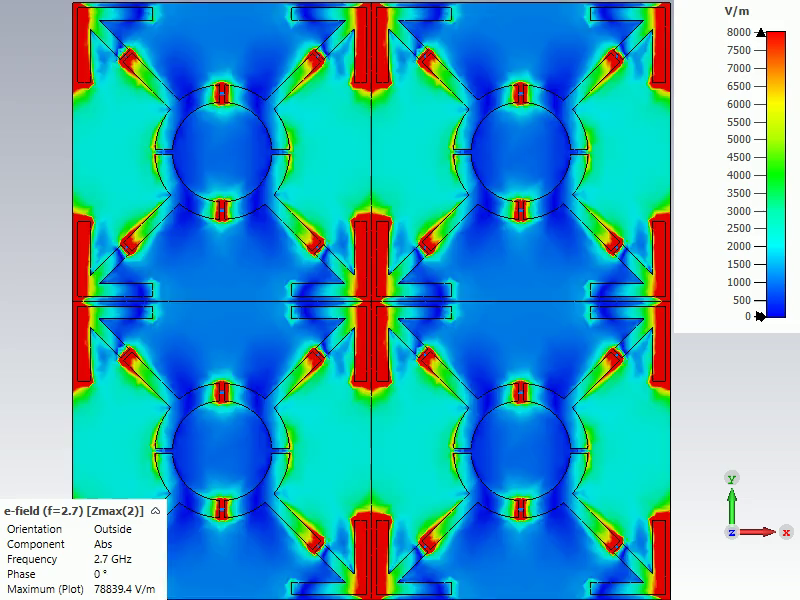
\includegraphics[page=1, width=0.22\textwidth]{E_Zmax2_027e2MHz.png}
            }{video/E_Zmax2_027e2MHz.mkv} \hfil
            \embedvideo{
                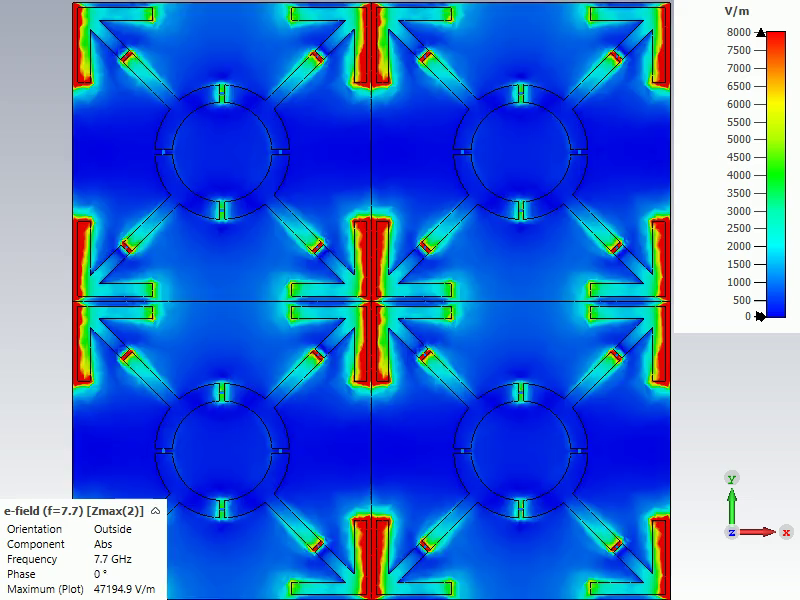
\includegraphics[page=1, width=0.22\textwidth]{E_Zmax2_077e2MHz.png}
            }{video/E_Zmax2_077e2MHz.mkv} \hfil
            \embedvideo{
                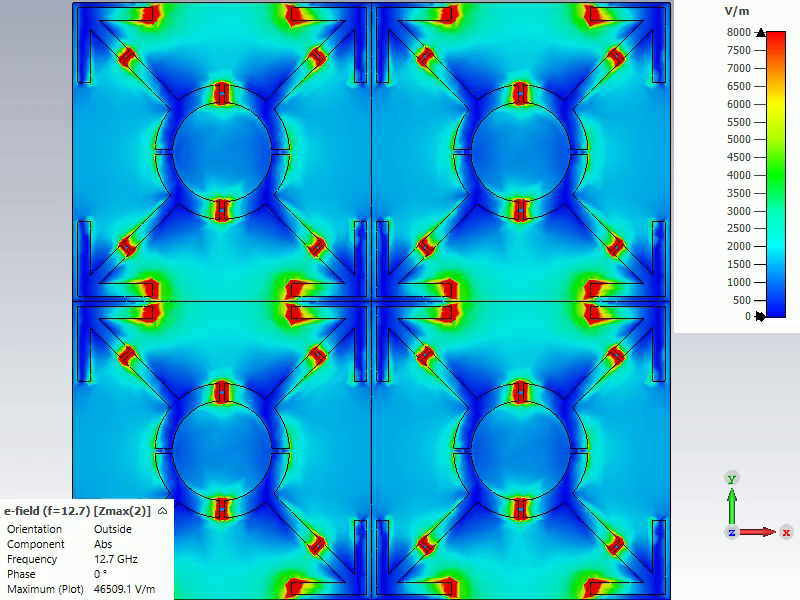
\includegraphics[page=1, width=0.22\textwidth]{E_Zmax2_127e2MHz.png}
            }{video/E_Zmax2_127e2MHz.mkv}

            \caption{Electrical Field for [2.7, 7.7, 12.7] GHz $Z_{max}(2)$}
            \label{img:E_Zmax2}
        \end{figure}


        Taking a look in the $S_{11}$ of $Z_{max}$ after the simulation as such (\ref{plt:S11_Zmax}).
        \begin{figure}[h]
            \centering
            \resizebox{\textwidth}{.5\textwidth}{%
                \begin{tikzpicture}
                    \begin{axis}
                        \addplot table[meta=s11] {data/s11.txt};
                    \end{axis}
                \end{tikzpicture}
            }
            \caption{\textsf{The $S_{11}$}}
            \label{plt:S11_Zmax}
        \end{figure}


    \subsection{\textsf{Alternative Modeling Methods}}
        In order to simulate the absorber there are also a few other ways to go about it:
        \begin{itemize}
            \item Transmission Line equivalent
            \item Electrical circuit equivalent
            \item Mathematical modeling \& code (MATLAB)
        \end{itemize}
        
        After having completed the simulation it is easy to extract the impedance of the
        absorber in order to try and implement the transmission line equivalent\dots